\chapter{Теоремы о промежуточных значениях непрерывной функции.}
\section{Промежуточные значения непрерывной функции на отрезке}

\begin{thm} [Больцано"--~Коши о промежуточных значениях\rindex{теорема!Больцано---Коши о промежуточных значениях}] \label{ch3n2}
Пусть функция~$f$ непрерывна на отрезке~$[a;b]$ и $f(a) = A$,~$f(b) = B$, тогда для любого~$C$, заключенного между~$A$ и~$B$, существует такая точка $c \in [a,b]$, что $f(c)=C$.
\end{thm}
Эту теорему можно переформулировать следующим образом.
\begin{thmn}[Больцано"--~Коши о промежуточных значениях] Непрерывная на отрезке функция, принимая какие-либо два значения, принимает и любое лежащее между ними значение. 
\end{thmn}
\begin{proof}
Пусть для определенности $f(a)=A < B = f(b)$ и тогда $f(a) < C < f(b)$.

Через $c_1$ обозначим середину отрезка $[a;b]$. Если $f(c_1) = C$, то искомая точка найдена и утверждение доказано.

Пусть $f(c_1)\ne C$. Тогда, если $f(c_1) > C$, то положим $a_1 = a$, $b_1 = c_1$, а если $f(c_1) < C$, то $a_1 = c_1$, $b_1 = b$, и поэтому всегда $f(a_1)<C<f(b_1)$.

По тому же самому принципу снова разделим отрезок $[a_1; b_1]$ пополам, и через $c_2$ обозначим его середину. Если $f(c_2) = C$, то утверждение доказано. Если же $f(c_2) \ne C$, то через $[a_2;b_2]$ обозначим ту половину, для которой $f(a_2) < C < f(b_2)$, и т.д. Процесс или обрывается на некотором шаге, и тогда утверждение доказано, или получается последовательность вложенных отрезков $\{[a_n;b_n]\}$ таких, что $\lim_{n \to \infty}\limits(b_n-a_n)=0$ и
\begin{equation}\label{ch3:th1:1}
f(a_n)<C<f(b_n)\quad \forall n\in \bbN.
\end{equation}

Таким образом, согласно  \hyperref[ch1:th:poslstyag]{теореме о последовательности стягивающихся отрезков} существует общая точка $c \in [a;b]$ всех отрезков $\{[a_n;b_n]\}$, причем 
$$
\lim_{n \to \infty}a_n = \lim_{n \to \infty}b_n = c.
$$

Поэтому в силу непрерывности функции~$f$ в точке~$c$:
\begin{equation}\label{ch3:th1:2}
\lim_{n \to \infty}f(a_n) = \lim_{n \to \infty}f(b_n) = f(c),
\end{equation}

Тогда из неравенств~\eqref{ch3:th1:1} в пределе при $n \to \infty$ следует 
\begin{equation}\label{ch3:th1:3}
\lim_{n \to \infty}f(a_n) \le C \le \lim_{n \to \infty}f(b_n),
\end{equation}
откуда из~\eqref{ch3:th1:2} и~\eqref{ch3:th1:3} получаем $f(c)=C$.

Случай, когда $A > B$, рассматривается аналогично.
 
Теорема доказана.
\end{proof}

\begin{cons}
Пусть функция~$f$ непрерывна на отрезке~$[a;b]$ и $f(a)$, $f(b)$ имеют разные знаки, тогда существует такая точка $c \in [a,b]$, что $f(c)=0$.
\end{cons}

\begin{thm}
Пусть функция $f$ непрерывна на отрезке~$[a;b]$ и $M=\sup f([a;b]) $, $m=\inf f([a;b])$. Тогда функция $f$ принимает все значения из отрезка $[m;M]$ и только эти значения.
\end{thm}
\begin{proof}
Согласно теореме~\ref{th:ch2:Veyershtrass} (Вейерштрасса) из прошлого билета существуют такие точки $\alpha\in [a;b]$ и $\beta\in [a;b]$, что $f(\alpha)=m$, $f(\beta)=M$

Тогда рассматриваемая теорема непосредственно вытекает из теоремы~\ref{ch3n2} (Больцано"--~Коши), примененной к отрезку $[\alpha;\beta]$, если $\alpha \le \beta$, или соответственно к отрезку $[\beta;\alpha]$, если $\beta \le \alpha$. 

Теорема доказана.
\end{proof} 

Таким образом, множество всех значений функции, заданной и непрерывной на некотором отрезке, представляет собой также отрезок. Однако, как показывают примеры, образом интервала может быть любой промежуток.

\section{Промежуточные значения непрерывной функции на промежутке}

Более точно отметим, что свойство непрерывных функций принимать все промежуточные значения справедливо для любого промежутка (конечного или бесконечного).

Но сначала заметим, что любой промежуток числовой прямой~$\bbR$ обладает следующим свойством: если $a\in\Delta$, $b\in\Delta$, $a<b$, то и $[a;b] \subset \Delta$. Очевидно, справедливо и обратное утверждение: если числовое множество обладает этим свойством, то оно является промежутком.

\begin{thm}
Если функция $f$ на промежутке $\Delta$ непрерывна и принимает значения~$A$ и $B$, $A<B$,  то она принимает и любое промежуточное значение $C\in (A;B)$.
\end{thm}
\begin{proof}
По условию, в промежутке~$\Delta$ существуют точки $a$ и $b$ такие, что $f(a) = A$, $f(b) = B$. Если, например, $a<b$, то тогда согласно теореме~\ref{ch3n2} (Больцано"--~Коши), рассматриваемая функция заведомо принимает указанное значение в некоторой точке отрезка~$[a;b]$, который является частью исходного промежутка~$\Delta$.
\end{proof} 

Другими словами, доказанная теорема утверждает, что если функция~$f$ непрерывна на промежутке~$\Delta$, и точки $a,b\in \Delta$ тогда для образа~$f(\Delta)$ выполняется следующее свойство: пусть $f(a)\in f(\Delta)$, $f(b)\in f(\Delta)$, $f(a)<f(b)$, то и $[f(a);f(b)]\subset f(\Delta)$. Это в точности указанное выше свойство промежутков. Значит, с помощью него эту теорему можно сформулировать следующим образом:	
\begin{thmn}
Если функция~$f$ непрерывна на промежутке~$\Delta$, то множество~$f(\Delta)$ является промежутком.
\end{thmn}

\section{Про обратное утверждение}
Заметим, что обратное утверждение является неверным, например, $f(x)= \sin\frac{1}{x}$ для $x\ne0$ и $f(0) = 0$ разрывна в точке $x = 0$, но у нее образ любого отрезка есть отрезок. Однако, для монотонных функций обратное утверждение является верным, докажем это в Теореме \ref{ch3n3}.

Однако, для дальнейших действий нам потребуются следующие определения.
\begin{defn}
Функция $f$ называется \textit{монотонно возрастающей \textup{(}убывающей) на множестве} $X \subset D_f$, если для любых $x_1$ и $x_2>x_1$ из множества $X$ 
$$
f(x_1)\le f(x_2) \quad (\text{соотв.}, f(x_1)\ge f(x_2)).
$$  
\end{defn}

\begin{defn}
Пусть $x_0$ "--- точка разрыва функции $f$. Тогда 
\begin{enumerate}[wide, labelwidth=!, labelindent=0pt]
\item
%\begin{figure}[!h]
%\centering
%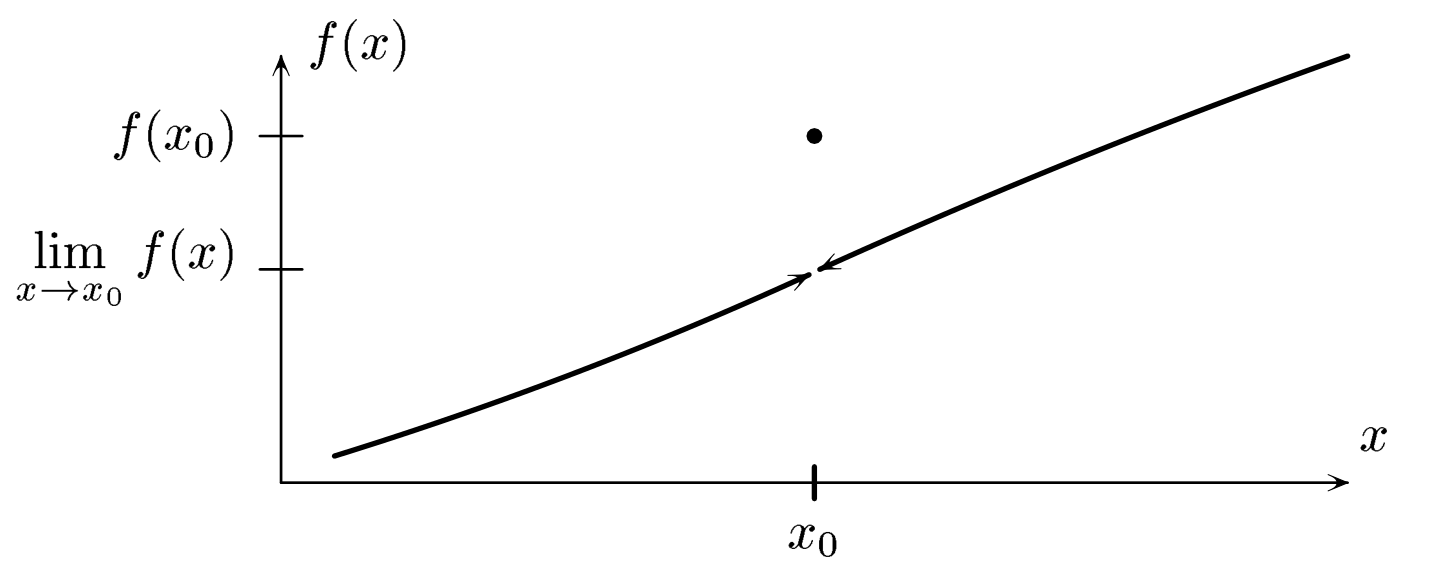
\includegraphics[width=0.7\textwidth]{pictures/ch3pict1}
%\end{figure}
%(что-то сделать с картинкой надо будет)

Если $\exists \lim_{x \to x_0}\limits f(x) \in \bbR$, то $x_0$ "--- \textit{точка устранимого разрыва}
\item
Если $\exists \lim_{x \to x_0\pm0}\limits f(x)=f(x_0\pm 0)$, но $f(x_0+0)\ne f(x_0-0)$, то $x_0$ "--- \textit{точка разрыва первого рода}, а число $\Delta f=f(x_0+0)-f(x_0-0)$ называется скачком функции $f$ в точке $x_0$.
\item
Все другие точки разрыва называют \textit{точками разрыва второго рода.} (т.е. хотя бы один из односторонних пределов либо не существует, либо бесконечен).
\end{enumerate}
\end{defn}
\begin{thm} \label{ch3n1} 
Если функция $f(x)$ определена и монотонна на интервале~$(a;b)$, то в каждой точке $x_0\in(a;b)$ она имеет односторонние пределы. Причем, если $f(x)$ "--- возрастающая, то 
$$
f(x_0-0)\le f(x_0)\le f(x_0+0),
$$
а если убывающая, то
$$
f(x_0-0)\ge f(x_0)\ge f(x_0+0).
$$
\end{thm}
\begin{thm} \label{ch3n3} 
Если функция $f$ определена и монотонна на промежутке $\Delta$ и $f(\Delta)$ — промежуток, то $f$ непрерывна на $\Delta$.
\end{thm}
\begin{proof}
Предположим противное, что функция $f$ разрывна в точке $x_0 \in\Delta$. Тогда по \hyperref[ch3n1]{теореме \ref{ch3n1}} в точке $x_0$ обязательно существуют односторонние пределы, значит $x_0$ не является точкой разрыва второго рода.  А в случае устранимой точки разрыва $f(x_0-0)=f(x_0+0)$, т.е.~отсюда и из неравенств из~\hyperref[ch3n1]{теоремы \ref{ch3n1}}, получим $f(x_0)=f(x_0-0)=f(x_0+0)$, т.е. функция непрерывна в точке разрыва, что невозможно. Значит $x_0$ не может быть точкой устранимого разрыва. Поэтому из монотонности следует, что $x_0$ может быть только точкой разрыва первого рода. Пусть, например, $f(x_0-0)\ne f(x_0)$.

Тогда $f$ не принимает значения, лежащие между $f(x_0 - 0)$ и $f(x_0)$, и поэтому $f(\Delta)$ не является промежутком, что противоречит условию. Следовательно, $f(x_0-0) = f(x_0)$. Аналогично доказывается, что  $f(x_0 + 0) = f(x_0)$, если, конечно, $x_0$ не является правым концом промежутка $\Delta$. 

Теорема доказана.
\end{proof} 